%% Bookheader, Nov 8, 2020; July 18, 2022

\documentclass[11pt]{../Support/ourbook}
%% or for landscape, comment out line above and use this one:
%%\documentclass[landscape,11pt]{ourbook}

%% This will keep space from stretching around display math:

\makeatletter
\renewcommand\normalsize{%
   \@setfontsize\normalsize\@xipt{13.6}%
   \abovedisplayskip 11\p@  \@minus6\p@
   \abovedisplayshortskip \z@ 
   \belowdisplayshortskip 6.5\p@ \@minus3\p@
   \belowdisplayskip \abovedisplayskip
   \let\@listi\@listI}
\makeatother
\normalsize


\begin{document}

\tableofcontents
\graphicspath{{../../Chapters/basic_spreadsheet/en_US}}
\chapter{Introduction to Spreadsheets}

Spreadsheets are the perfect
tool for many real world problems. In this chapter, you will be introduced to how to use a
spreadsheet. There are numerous spreadsheet programs, such as Google Sheets,
Microsoft Excel, Apple Numbers, and OpenOffice Calc.  All of them are
relatively similar. This instruction will use Google Sheets, but if you are using one
of the others, you should be able to follow along.

The first spreadsheet program (VisiCalc) was introduced in 1979 as a
tool for finance people to play ``what if'' games.  For example, a
company might make a spreadsheet that told them how much more profit
they would make if they changed from using an expensive metal to using
a cheaper alloy.\index{Spreadsheet}

In honor of this history, let's start by studying a business question:
You have a friend who dreams of quitting her job to become a cooper. (A
cooper makes barrels that are used for aging wine and whiskey.)  According to her:
\begin{itemize}
\item It costs \$45 dollars in materials to build one barrel.
\item A barrel sells for \$100 dollars.
\item The workshop/warehouse she wants to rent costs \$2000 per month.
\item Taxes take 20\% of her profits.
\item She needs to make \$4000 monthly after taxes.
\end{itemize}

She has asked you, ``How many barrels do I need to make each month?''


\section{Solving It Symbolically}

Many problems can be solved two ways: symbolically or
numerically.\index{symbolic vs. numeric solutions} To solve this
problem symbolically, you would write out the facts as equations or
inequalities, then do symbol manipulations until you ended up with
an answer. In this case, you would let $b$ be the number of barrels
and create the following inequality:

$$(1.0 - 0.2)\left(b(100 - 45) - 2000\right) \geq 4000$$

You would simplify it:

$$(0.8)\left(55 b - 2000\right) \geq 4000$$

And simplify it more:

$$44b - 1600 \geq 4000$$

If that is true, then:

$$44b \geq 5600$$

And if that is true, then:

$$b \geq \frac{1400}{11}$$

$1400/11$ is about 127.27, so she needs to make and sell 128 barrels
each month.

That is a perfect answer, and we didn't need a spreadsheet at all. However:
\begin{itemize}
\item As problems get larger and more realistic, it gets much more difficult to solve them symbolically.
\item As soon as you say ``Yes, you need to make and sell 128 barrels
  each month.'' Your friend will ask ``What if I make and sell 200
  barrels? How much money will I make then?''
\end{itemize}

So, we use a spreadsheets to solve the problem numerically.

\section{Solving It Numerically (with a spreadsheet)}


Let's get back to our example. Put labels in the A column:
\begin{itemize}
\item{Barrels produced (per month)}
\item{Materials cost (per barrel)}
\item{Sale price (per barrel)}
\item{Pre-tax earnings (per month)}
\item{Taxes (per month)}
\item{Take home pay (per month)}
\end{itemize}

Format them any way you like. It should look something like this:

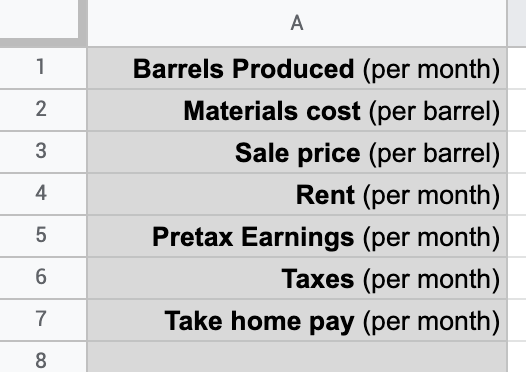
\includegraphics[width=0.4\textwidth]{BarrelLabels.png}

In the B column, the first four cells are values (not formulas):
\begin{itemize}
\item{115 formatted as a number with no decimal point}
\item{45 formatted as currency}
\item{100 formatted as currency}
\item{2000 formatted as currency}
\end{itemize}

It should look something like this:

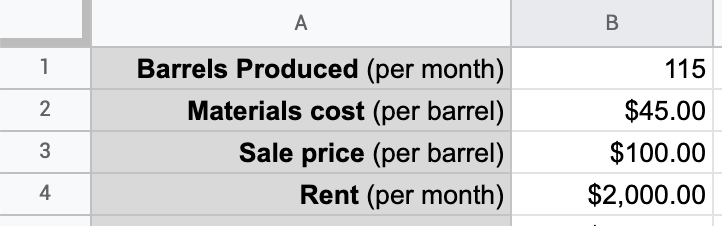
\includegraphics[width=0.5\textwidth]{BarrelValues.png}

The next three cells in the B column will have formulas:
\begin{itemize}
\item{B1 * (B3 - B2) - B4}
\item{0.2 * B5}
\item{B5 - B6}
\end{itemize}

It should look something like this:

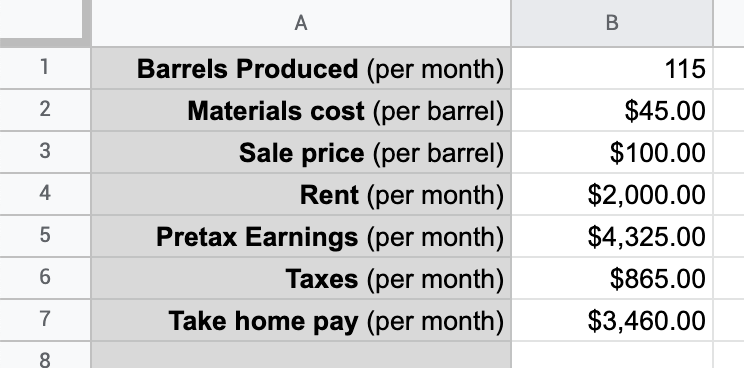
\includegraphics[width=0.5\textwidth]{BarrelFormulas.png}

Now you can share this spreadsheet with your friend, and she can put
different values into the cells for what-if games, such as ``If I can
get my materials cost down to \$42 per barrel, what happens to my take
home pay?''

Sometimes it is nice to show a range of values for a variable or two.
In this case, it might be nice to show your friend what the numbers
look like if she produces 115, 120, 125, 130, 135, or 140 barrels per
month.

We have one column, and now we need six. How do we duplicate cells?
\begin{enumerate}
\item Click B1 to select it, then shift-click on B7 to select all seven cells.
\item Copy them. (Depending on what program you are using, there is likely a menu item for this.)
\item Click C1 to select it
\item Paste them.
\end{enumerate}

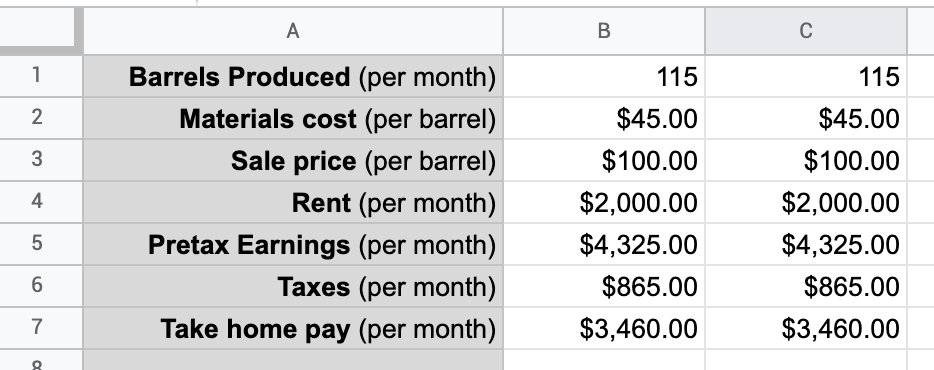
\includegraphics[width=0.5\textwidth]{BarrelCopyPaste.png}

We want the first cell in the new column to be 120. You could just
type in 120, but let's do something more clever. Put a formula into that
cell: = B1 + 5.  Now, the cell should show 120.

Why did we put in a formula? When we duplicate this column, this cell
will always have 5 more barrels than the cell to its left.

Next, let's duplicate the second column a few times. The easy way to do
this is to select the cells as you did before, then drag the lower-right
corner to the right until column G is in the selection. When you end
the drag, the copies will appear:

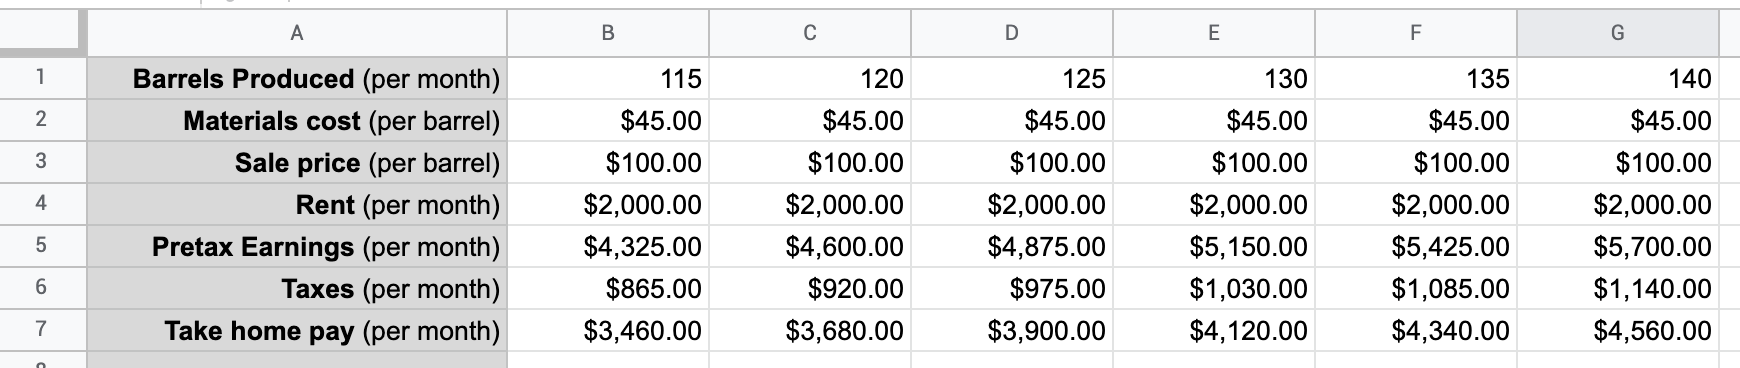
\includegraphics[width=0.8\textwidth]{BarrelDragPaste.png}

Nice, right? Now your friend can easily see how many barrels
correspond to how much take-home pay. But do you know what would be even more helpful? A graph.

\section{Graphing}

Graphing is a little different on every different platform.  Here is what you want the graph to look like:

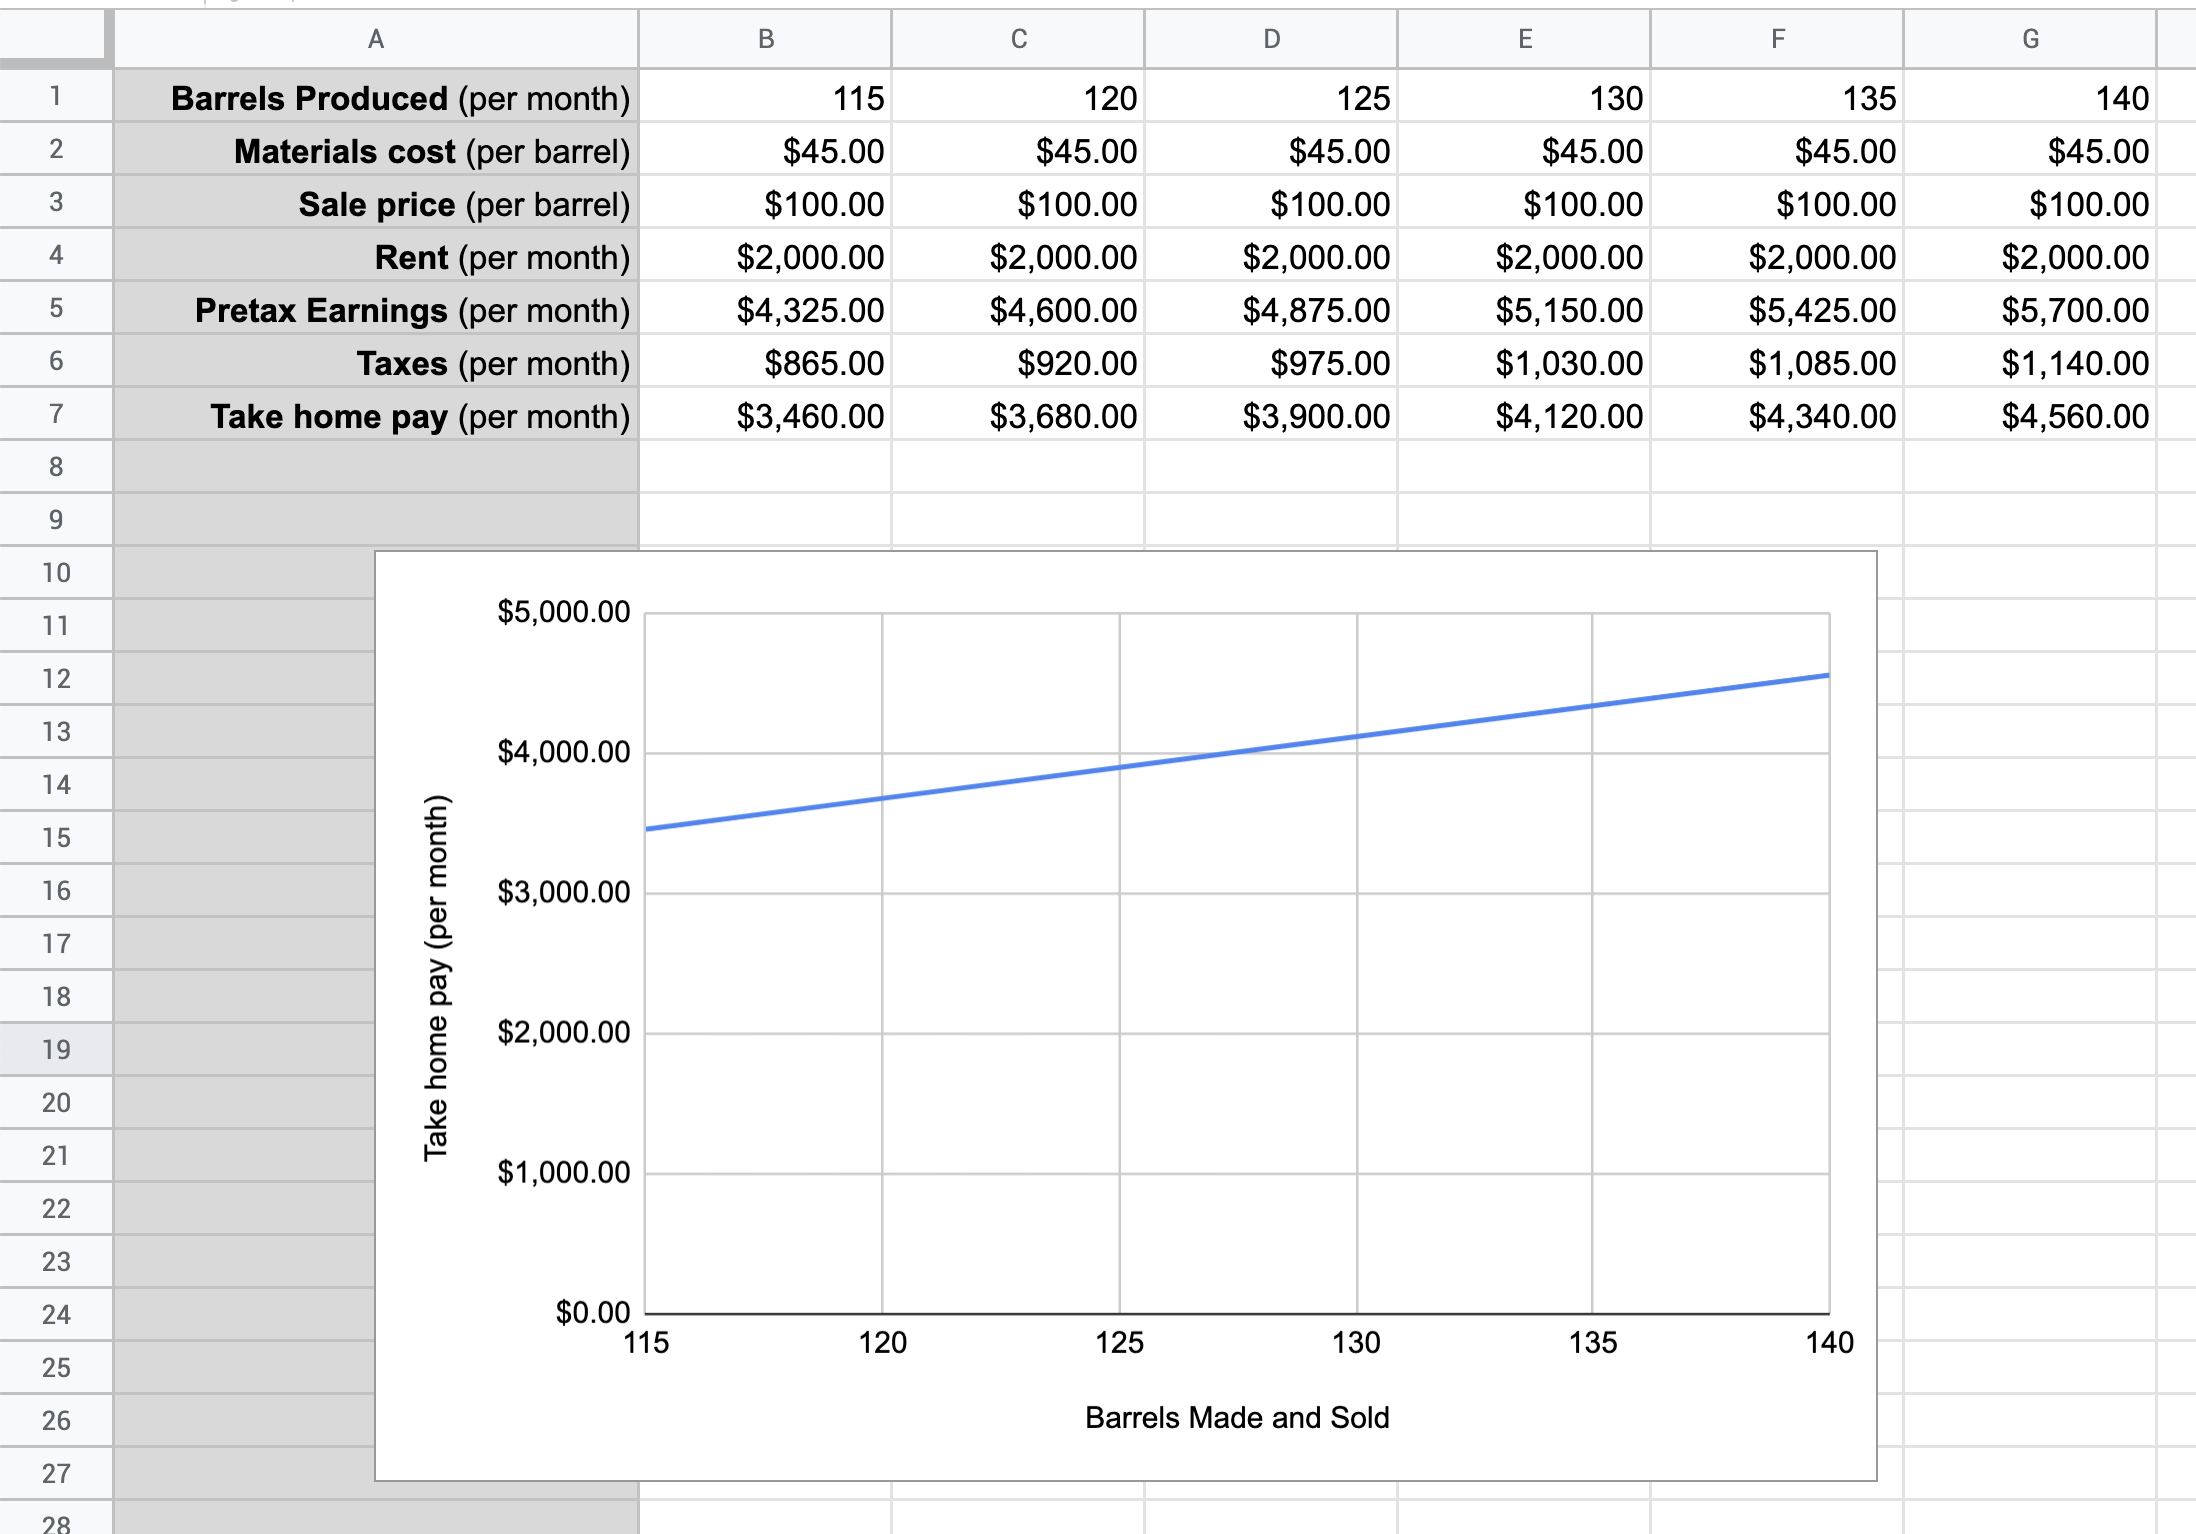
\includegraphics[width=0.8\textwidth]{BarrelGraph.png}

On Google Sheets:\index{spreadsheet!graphs}

\begin{enumerate}
\item Select cells B7 through G7. 
\item Choose the menu item Insert -> Chart.
\item Choose the chart type (Line)
\item Add the X-axis to be B1 through G1.
\item Under the Customize tab, Set the label for the X-axis to be ``Barrels Made and Sold''.
\item Delete the chart title (which is the same as the Y-axis label).
\end{enumerate}

\section{Other Things You Should Know About Spreadsheets}

Your spreadsheet document can have several ``Sheets''.  Each has its
own grid of cells.  The sheet has a name; usually, you call it
something like ``Salaries''.  When you need to use a value from the
``Salaries'' sheet in another sheet, you can specify ``Salaries!A2''
--- that is, cell A2 on sheet ``Salaries''.  To flip between the sheets,
there is usually a tab for each at the bottom of the document.

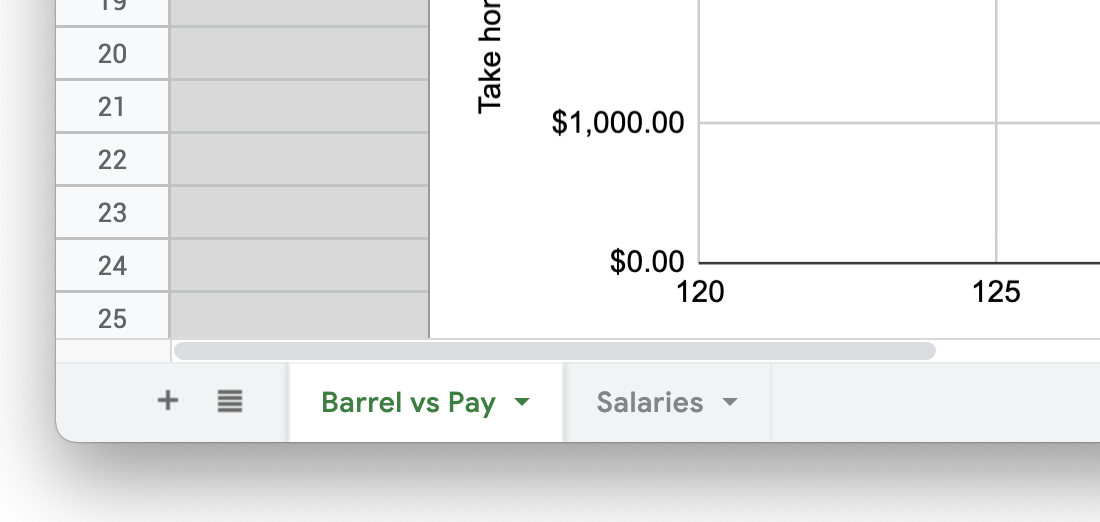
\includegraphics[width=0.5\textwidth]{Sheets.png}

By default, the cell references are relative. In other words, when you write
a formula in cell H5 that references the value in cell G4, the cell
remembers ``The cell that is one up and one to the left of me.''
Thus, if you copy that formula into B9, now that formula reads the
value from A8.

If you want an absolute reference, you use \$. If H5 references
\$G\$4, G4 will be used no matter where on the sheet the formula is
copied to.

You can use the \$ on the row or column. In \$A4, the column is
absolute and the row is relative.  In A\$4, the row is absolute and
the column is relative.

\section{Challenge: Make a spreadsheet}

You have a company that bids on painting jobs. Make a
spreadsheet to help you do bids. Here are the parameters:
\begin{itemize}
\item The client will tell you how many square meters of wall needs to be painted.
\item Paint costs \$0.02 per square meter of wall
\item On average, a square meter of wall takes 0.02 hours to paint.
\item You can hire painters at \$15 per hour.
\item You add 20\% to your estimated costs for a margin of error and profit.
\end{itemize}

Make a spreadsheet such that when you type in the square meters to be
painted, the spreadsheet tells you how much you will spend on paint
and labor.  It should also tell you what your bid should be.

\graphicspath{{../../Chapters/compound_interest/en_US}}
\chapter{Compound Interest}

When you loan money to someone, you typically charge them some sort of
interest. The most common loan of this sort is what the bank calls a
``savings account''.  Any money you put in the account is loaned to
the bank. The bank then lends it to someone else, who pays interest to
the bank. The bank gives some of that interest to you.
% Diagram needed
However, what if you leave the interest in your account? And you start
making \textit{interest on the interest}? This is known as
\textit{compound interest}.\index{compound interest}

\section{An example with annual interest payments}

Let's say that you put \$1000 in a savings account that pays 6\%
interest every year. How much money would you have after 12 years?
Let's make a spreadsheet.

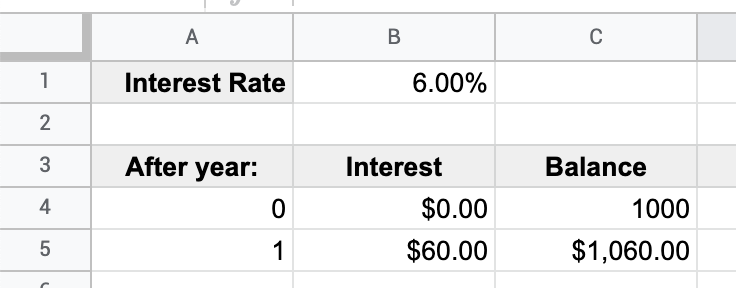
\includegraphics[width=0.4\textwidth]{StartInterest.png}

Create a new spreadsheet and edit the cells to look like this.  All
the cells in rows 1 - 4 are just values: just type in what you
see.

The fifth row is all formulas:

\begin{tabular}{c | c | c}
  After year & Interest & Balance \\
  \hline 
  = A4 + 1 & = B\$1 * C4 & = C4 + B5 \\
\end{tabular}

The interest rate field should be formatted as a percentage. One thing
to know when dealing with percentages in the spreadsheet: If the field
says ``600\%'', its value is 6. 

The cells in the Interest and Balance column should be formatted as currency.

You are about to make several copies of the cells in the fifth row,
so make sure they look right.

Click on A5 and shift-click on C5 to select all three cells. Drag the
lower-right corner down to fill the rows 6 - 15.

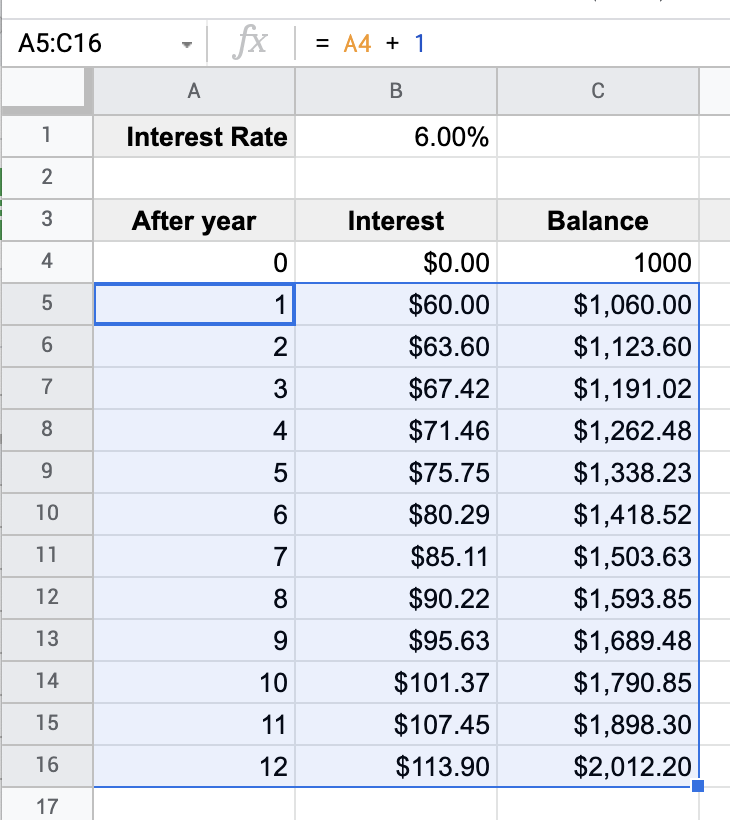
\includegraphics[width=0.5\textwidth]{CopiedCellsInterest.png}

Look at the numbers.  The first interest payment is \$60, but the last
is \$113.90. Your balance has more than doubled!

\section{Exponential Growth}

We figured this out numerically by repeatedly multiplying the balance
by the interest rate. What if you wanted to know what the balance
would be $n$ years after investing $P_0$ dollars with an annual interest
rate of $r$? (Note that $r$ in our example would be 0.06, not 6.0.)

Each year, the balance is multiplied by $1 + r$, so after one year,
$P_0$ would become $P_0 \times (1 + r)$.  The next year you would multiply
this number by $(1 + r)$ again: $P_0 \times (1 + r) \times (1 + r)$. The
next year? $P_0 \times (1 + r) \times (1 + r) \times (1 + r)$ See the
pattern? $P_n$ is this balance after $n$ years, then

$$P_n = P_0 (1+r)^n$$

Because $n$ is an exponent, we call this \textit{exponential growth}.
There are few things as terrifying to a scientist as
the phrase ``The population is undergoing exponential growth''.\index{exponential growth}
% Diagram/ Explain

\section{Sensitivity to interest rate}

For most people, the first surprising thing about compound interest is
how quickly your money grows after a few years.  The second thing that
is surprising is how much difference a small change in the percentage
rate makes.

Let's add another set of columns that shows what happens to your money
if you convince the bank to pay you 8\% instead of 6\%.

Copy everything from columns B and C:

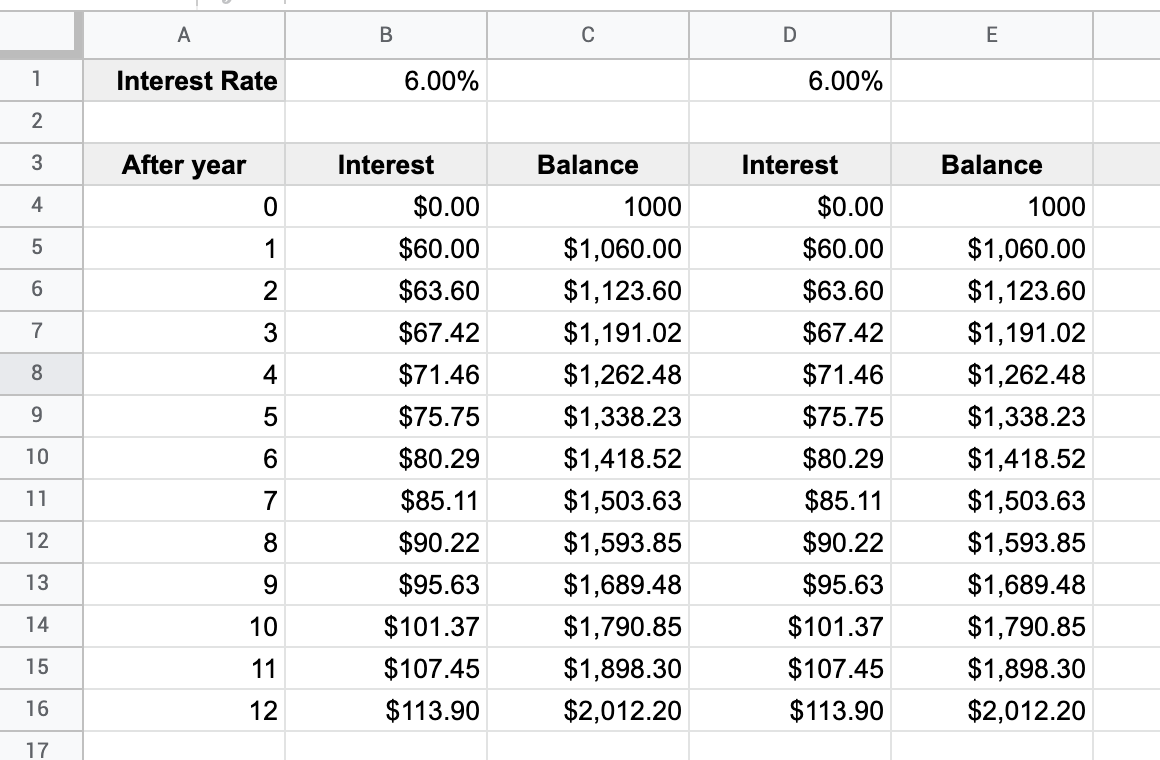
\includegraphics[width=0.6\textwidth]{CopyForSecondInterest.png}

Now edit the second interest rate to be 8\%:

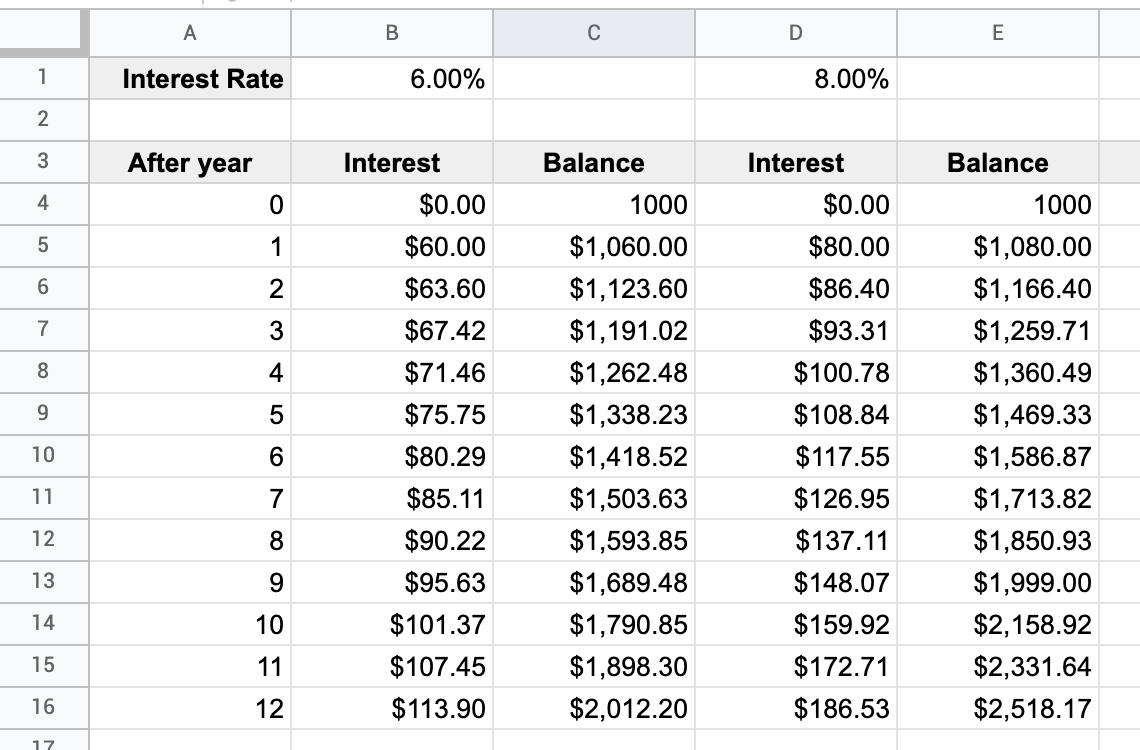
\includegraphics[width=0.6\textwidth]{AtBiggerInterestRate.png}


\graphicspath{{../../Chapters/intro_dataviz/en_US}}
\chapter{Introduction to Data Visualization}

It is difficult for the human mind to look at a list of numbers and
identify the patterns in them, so we often use these numbers to make a picture. These pictures are called \textit{graphs},
\textit{charts}, or \textit{plots}. Often, the right picture can make
the meaning in the data obvious. \textit{Data visualization} is the
process of making pictures from numbers.

\section{Common Types of Data Visualizations}

Depending on the type of data and what you are trying to demonstrate
about it, you will use different types of data visualizations.  How
many types of data visualizations are there? Hundreds, but we will
concentrate on just four: The bar chart, the line graph, the pie
chart, and the scatter plot.

\subsection{Bar Chart}

Here is an example of a bar chart.\index{bar chart}

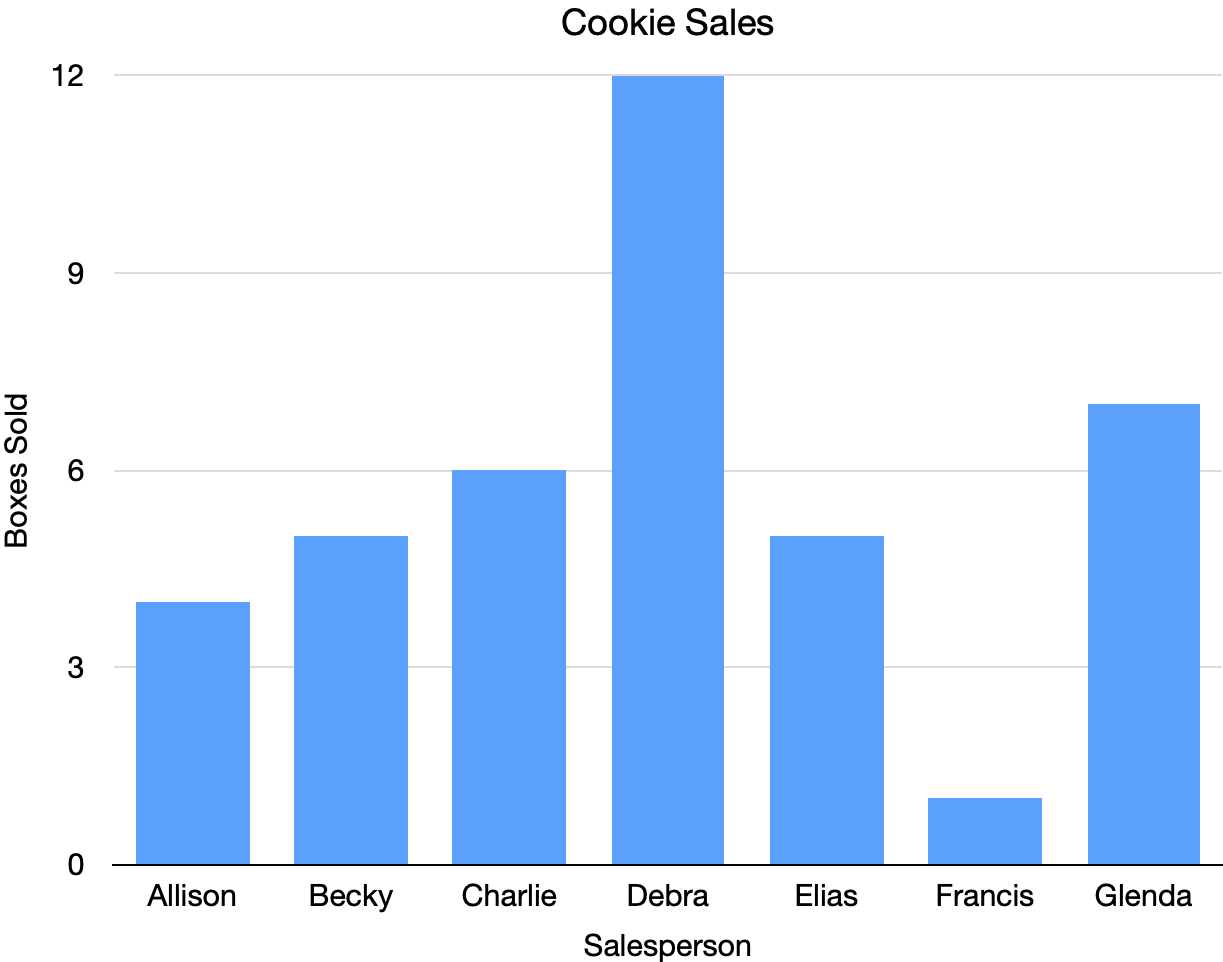
\includegraphics[width=0.7\textwidth]{CookieChart.png}

Each bar represents the cookie sales of one person. For example,
Charlie has sold 6 boxes of cookies, so the bar goes over Charlie's
name and reaches to the number 6.

Looking at this chart, you probably think, ``Wow, Debra has sold a lot
more cookies than anyone else, and Francis has sold a lot fewer.''

The same data could be in a table like this:

\begin{tabular}{c | c}
  Salesperson & Boxes Sold \\
  \hline
  Allison & 4 \\
  Becky & 5 \\
  Charlie & 6\\
  Debra & 12\\
  Elias & 5\\
  Francis & 1\\
  Glenda & 7
\end{tabular}

A table (especially a large table) is often just a bunch of
numbers. A chart helps our brains understand what the numbers mean.

Bar charts can also go horizontally.

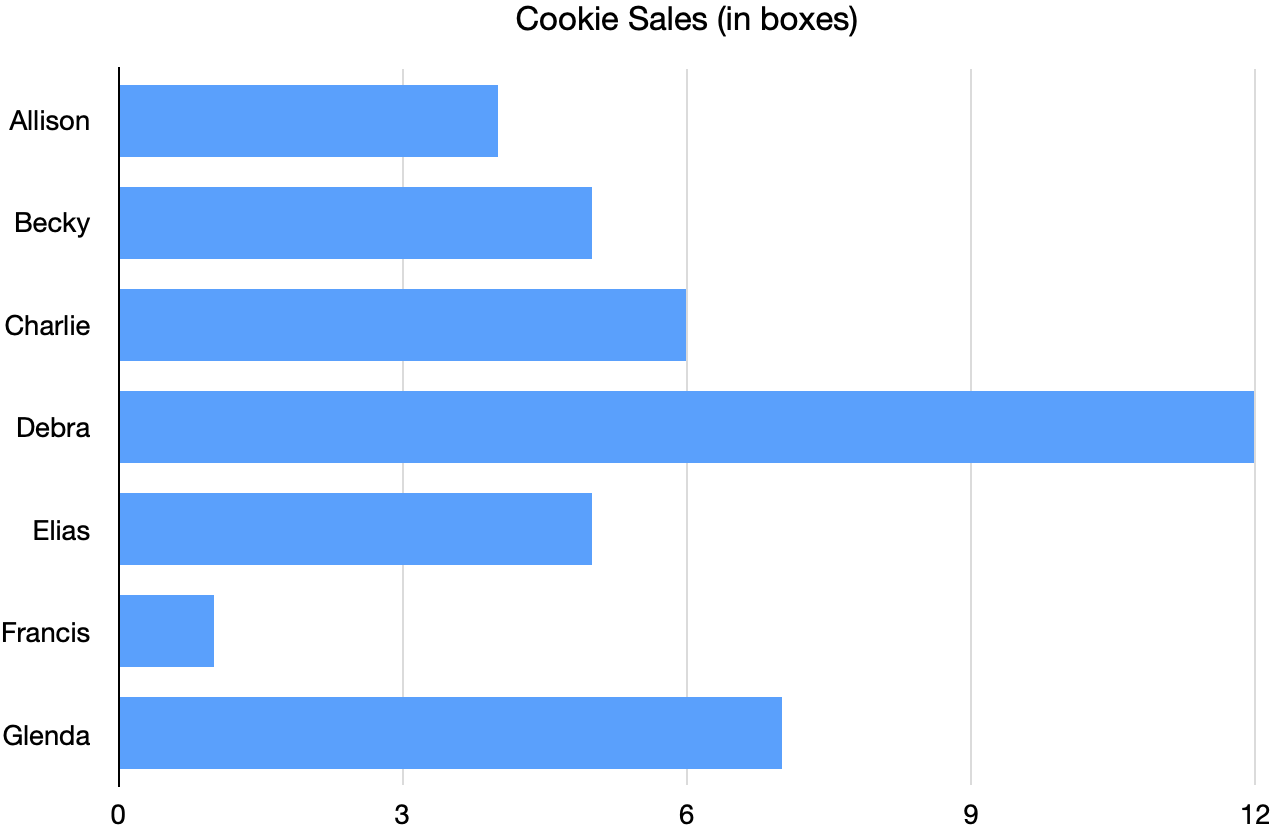
\includegraphics[width=0.7\textwidth]{HorizontalBarCookies.png}

Sometimes we use colors to explain what contributed to the number.

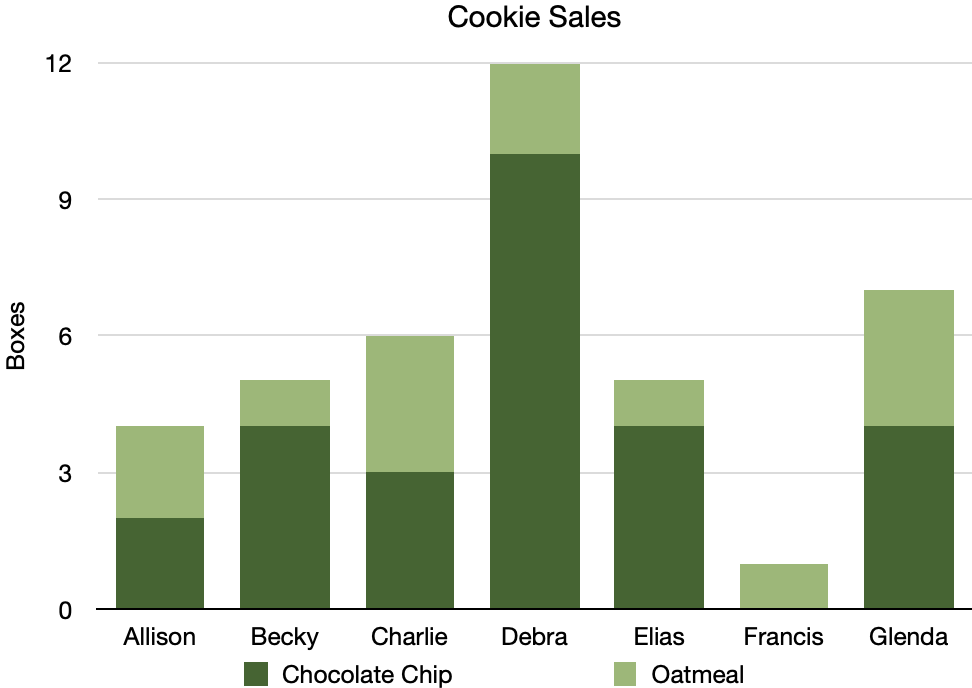
\includegraphics[width=0.7\textwidth]{TypesCookieBar.png}

This tells us that Becky sold more boxes of chocolate chip cookies
than boxes of oatmeal cookies.

\subsection{Line Graph}

Here is a line graph:\index{line graph}

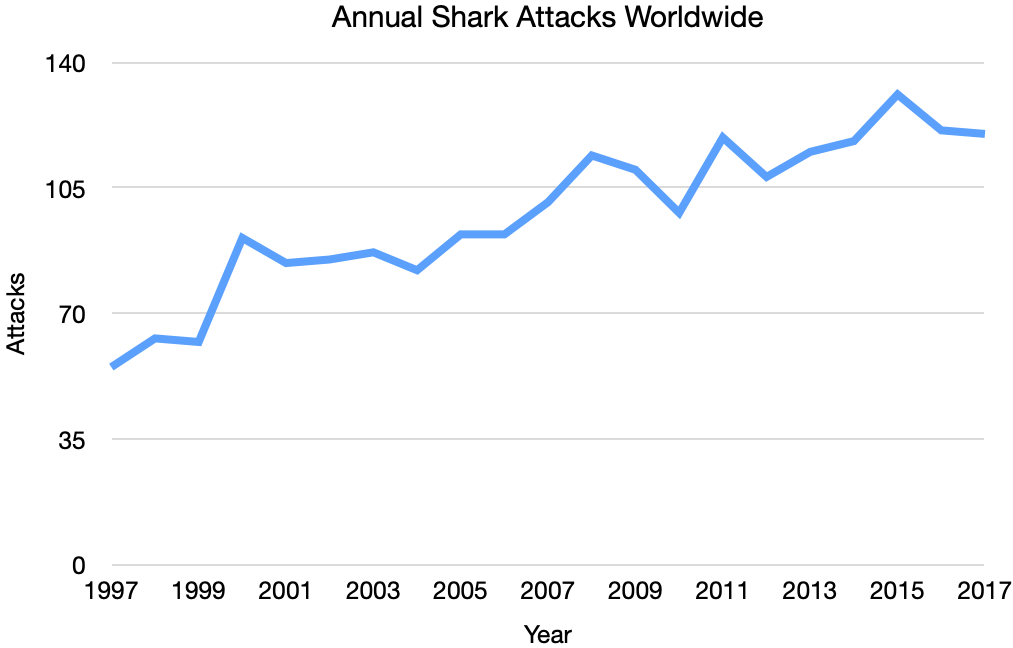
\includegraphics[width=0.7\textwidth]{SharksLine1.png}

These are often used to show trends over time. Here, for example, you
can see that the number of shark attacks has been increasing over
time.

You can have more than one line on a graph.

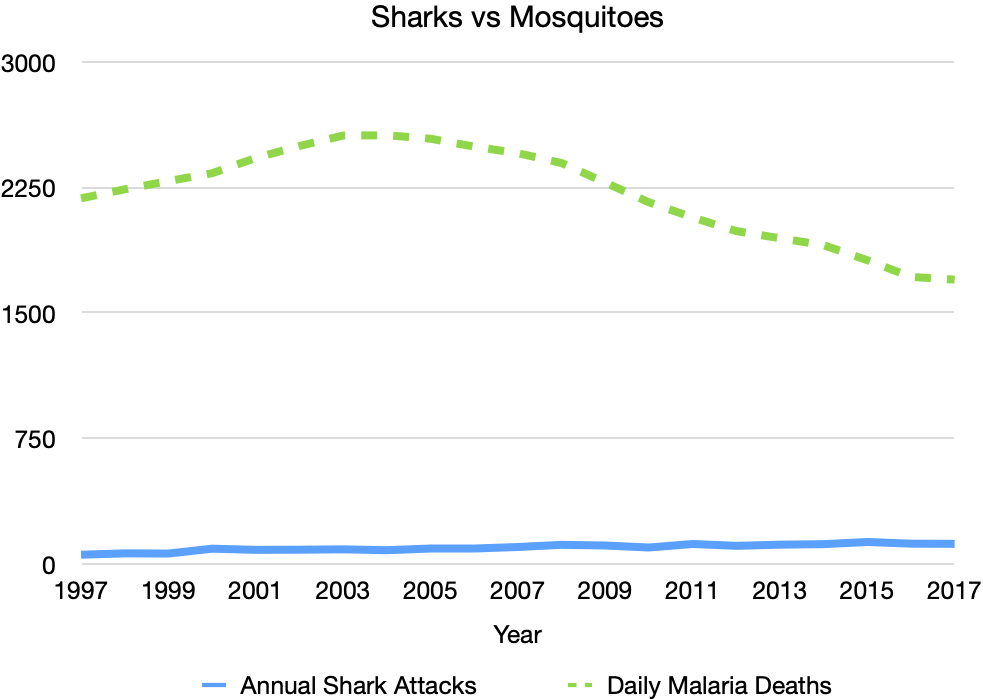
\includegraphics[width=0.7\textwidth]{SharksVsMosquitoes.png}

\subsection{Pie Chart}

You use a pie chart when you are looking at the comparative size of numbers.\index{pie chart}

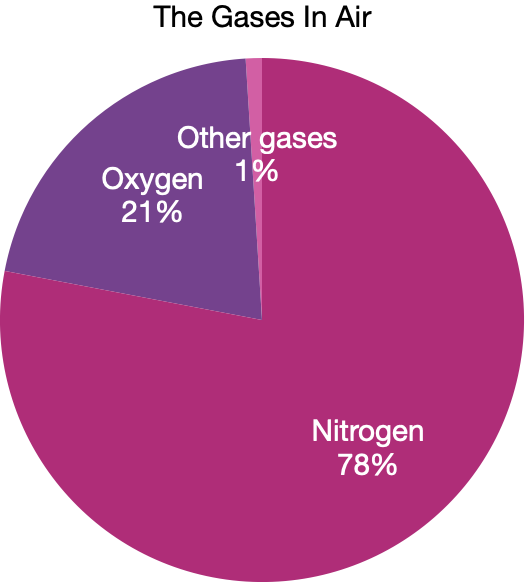
\includegraphics[width=0.4\textwidth]{AirPie.png}

\subsection{Scatter Plot}

Sometimes, you have a large number of data points with two values, and you are
looking for a relationship between them.  For example, maybe you write
down the average temperature and the total sales for your lemonade
stand on the 15th of every month:\index{scatter plot}

\begin{tabular}{c | c | c}
  Date &	Avg. Temp. &	Total Sales \\
  \hline
15 January 2022 & 2.6º C & \$183.85 \\
15 February 2022 & -4.2º C & \$173.56\\
15 March 2022 & 13.3º C & \$195.22\\
15 April 2022 & 26.2º C & \$207.61\\
15 May 2022 & 27.5º C & \$210.88\\
15 June 2022 & 31.3º C & \$214.18\\
15 July 2022 & 33.5º C & \$215.23\\
15 Aug 2022 & 41.7º C & \$224.07\\
15 September 2022 & 20.7º C & \$198.94\\
15 October 2022 & 17.2º C & \$196.10\\
15 November 2022 & 1.7º C & \$185.10\\
15 December 2022 & 0.2º C & \$188.70 \\
\end{tabular}

You may wonder, "Do I sell more lemonade on hotter days?''

To figure this out, you might create a scatter plot.  For each day, you put a mark that
represents that temperature and the sales that day:

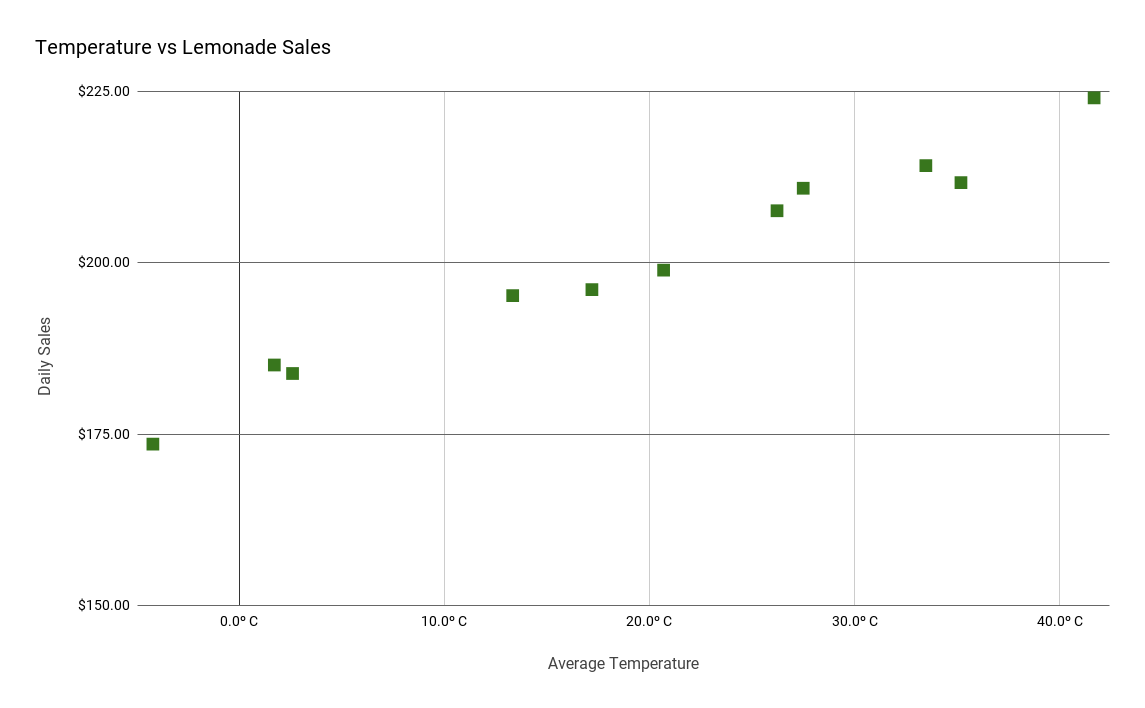
\includegraphics[width=\textwidth]{LemonadeScatter.png}

From this scatter plot, you can easily see that you do sell more
lemonade as the temperature goes up.


\section{Make Bar Graph}

Go back to your compound interest spreadsheet and make a bar graph
that shows both balances over time:

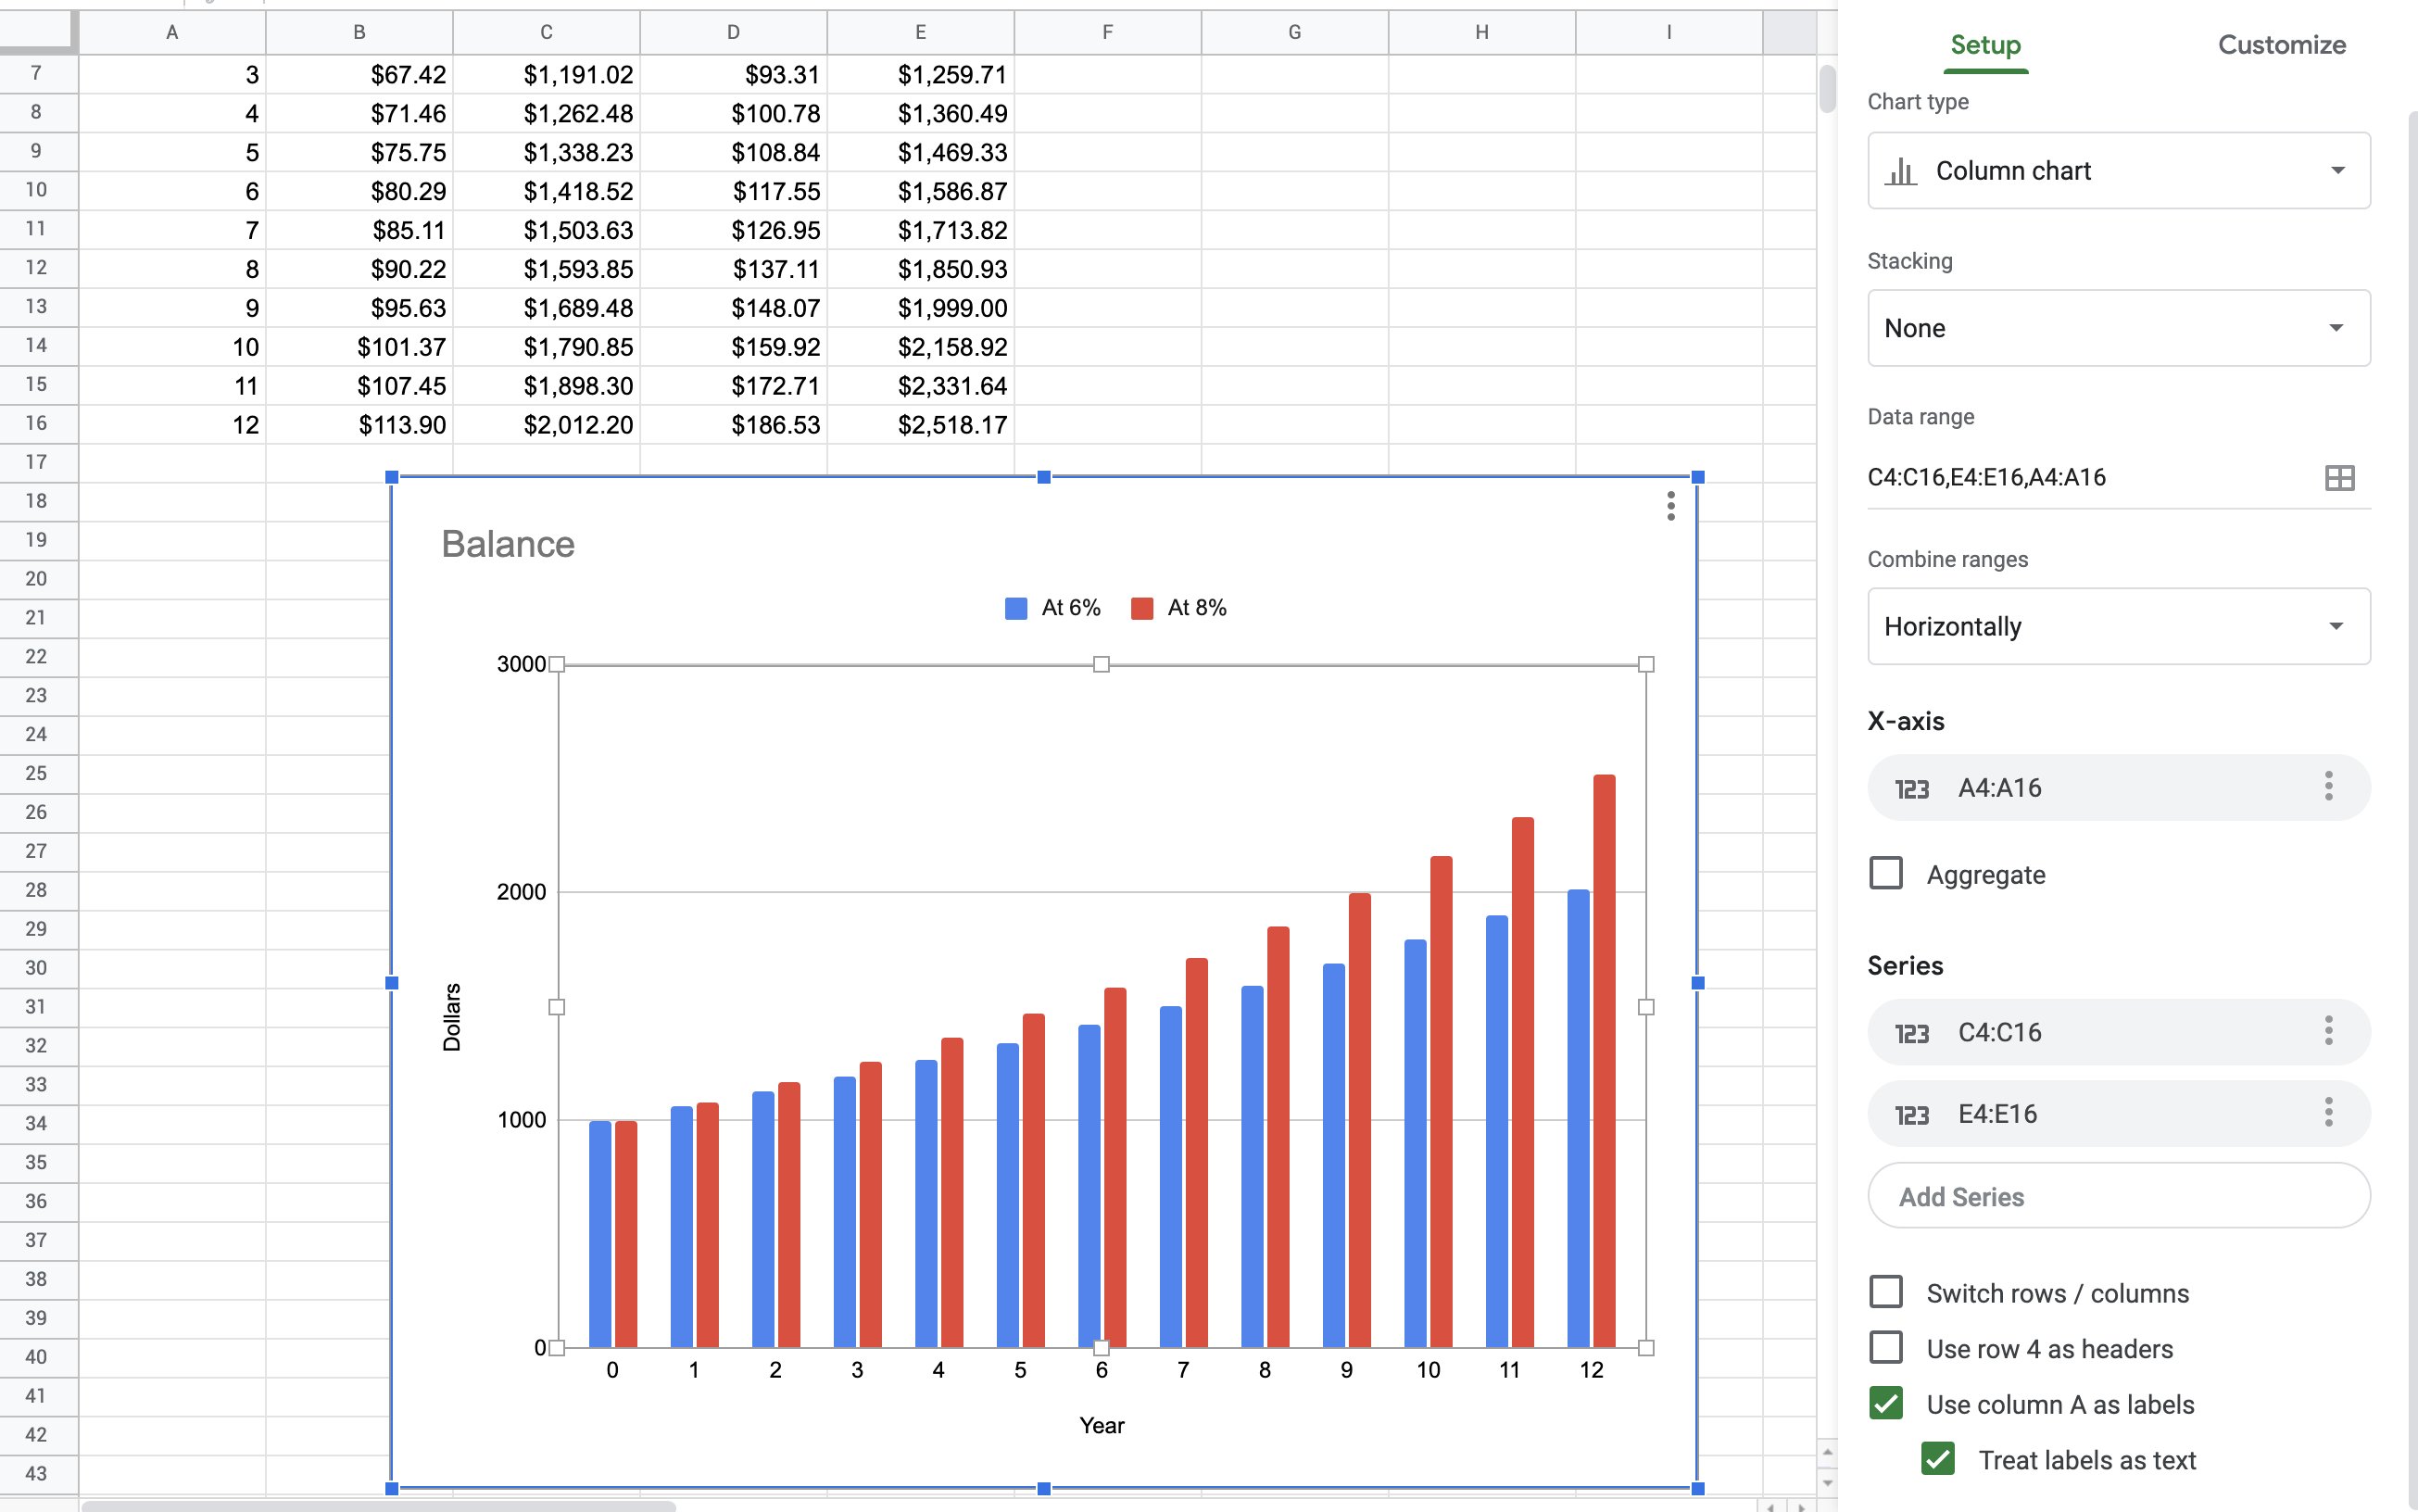
\includegraphics[width=0.9\textwidth]{InterestGraph.png}

The year column should be used as the x-axis. There are two series of
data that come from C4:C16 and E4:E16.  Tidy up the titles and legend
as much as you like.\index{spreadsheet!graphing multiple series}

Looking at the graph, you can see the balances start the same, but
balance of the account with the larger interest rate quickly pulls
away from the account with the smaller interest rate.


%%%%%%%%%%%%%%%%%%%%%%%%%%%%%%%%%
%% Bookfooter.tex by Aaron Hillegass
%% Nov 8, 2020

\appendix

\chapter{Answers to Exercises}
\shipoutAnswer

\bibliography{references}

\printindex

\end{document}